\chapter{ƯỚC TÍNH TỌA ĐỘ KHUNG XƯƠNG TRÊN ẢNH RGB BẰNG MẠNG MOBILENET-V2}
\label{s:pose estimate}
Trong nội dung này, em sẽ trình bày hai phương pháp đề xuất để trích xuất đặc trưng khung xương. Đó là trích xuất đặc trưng từ thiết bị Kinect và trích xuất đặc trưng từ mạng neuron network. Phương pháp trích xuất đặc trưng khung xương từ ảnh RGB qua mạng mobilenet v2 được áp dụng trong đề tài vì tính khả thi, có thể ứng dụng được trong đời sống bằng cách tích hợp lên điện thoại thông minh.

\section{ƯỚC TÍNH DỰA TRÊN CAMERA ĐỘ SÂU KINECT}
\label{ss:kinect}
\subsection{Giới thiệu camera cảm biến độ sâu Kinect của Microsoft}
Kinect là một thiết bị đầu vào,là cảm biến chuyển động do hãng Microsoft sản xuất dành cho Xbox 360 và máy tính Windows. Dựa trên một webcam kiểu add-on ngoại vi cho Xbox 360, nó cho phép người dùng điều khiển và tương tác với Xbox 360 mà không cần phải dùng đến một bộ điều khiển tay cầm, thông qua một giao diện người dùng tự nhiên bằng cử chỉ và lệnh nói. Thiết bị được giới thiệu vào tháng 11 năm 2010 như một phụ kiện của Xbox 360. Cảm biến chiều sâu (depth sensor) được sử dụng trong Kinect được lấy từ việc trích xuất camera hồng ngoại. 

Chức năng chính của Kinect là một công cụ để người dùng tương tác với Xbox 360 bằng cử chỉ và lệnh nói. Vì lý do này, các bộ cảm biến có khả năng thu thập dữ liệu ở độ phân giải 640x480 điểm ảnh. Với các dữ liệu chiều sâu, có thể lấy được "các vector đặc trưng mang hình dáng của khung xương con người(SJM)" của người đứng phía trước của cảm biến. Và với các SJM đó, nó có thể nhận biết được cử chỉ của người sử dụng.

\FloatBarrier
\begin{figure}[htp]
\begin{center}
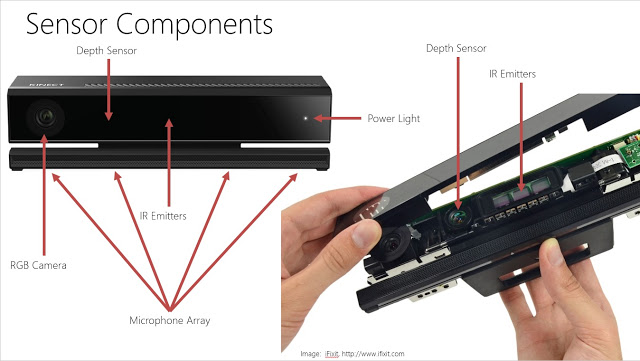
\includegraphics[scale=0.8]{chap3/c3_figs/kinect.png}
\end{center}
\caption{Camera cảm biến độ sâu Kinect \\Nguồn : \url{https://www.ifixit.com}}
\label{fig:kinect}
\end{figure}
\FloatBarrier

Các thông số cơ bản của cảm biến như sau:
\begin{itemize}
\item Ảnh màu : 1920x1080 @30Hz (15Hz ánh sáng yếu)
\item Ảnh độ sâu : 512x424 @30Hz
\item Tầm xa : 0.5 $\sim$ 4.5m
\item Góc nhìn (Dọc/Ngang) : 70 / 60 độ
\item Số lượng SJM (phát hiện/theo dõi) : 6 / 6 SJMs
\item Số lượng SJM-J : 25 SJM-Js
\item Hệ điều hành : Windows 8/10
\item Cổng tín hiệu : USB 3.0
\end{itemize}

Cơ chế hoạt động: Ban đầu, bộ phần phát tia hồng ngoại sẽ phát ra tia hồng ngoại trong vùng hoạt động của nó. Thông qua phản chiếu các tia hồng ngoại về camera hồng ngoại sẽ thu nhận được các tia phản xạ về. Dựa vào thời gian trễ để đo khoảng cách tới các điểm trong vùng quan sát. Kết quả thu về sẽ là hình ảnh vùng quan sát với những chiều sâu khác nhau.

\FloatBarrier
\begin{figure}[htp]
\begin{center}
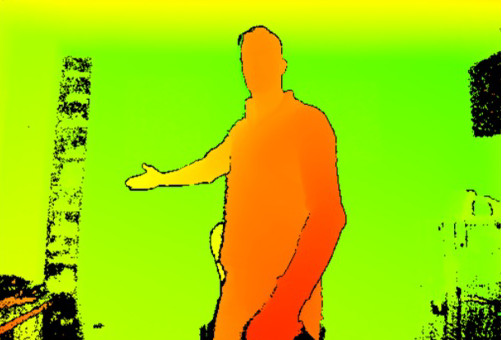
\includegraphics[scale=0.8]{chap3/c3_figs/depth.jpg}
\end{center}
\caption{Ảnh độ sâu từ Kinect \\(Nguồn : \url{https://www.zonetrigger.com/)}}
\label{fig:kinect}
\end{figure}
\FloatBarrier

\subsection{Cơ chế trích xuất SJM từ Kinect}


\section{ƯỚC TÍNH TỪ ẢNH 2D DỰA TRÊN MẠNG NEURAL NETWORK}
\label{ss:2Dpose}
\subsection{Tổng quan phương pháp}
\label{sss:tong_quan_2D_pose}
Phương pháp trích xuất hình dáng khung xương được áp dụng từ bài báo "Realtime Multi-Person 2D Pose Estimation using Part Affinity Fields" \cite{cao2017realtime} sử dụng phương pháp bottom-up ước tính tọa độ khung xương từ ảnh sang không gian 2D. Tuy có rất nhiều mạng pose estimate cả 2D lẫn 3D và cả dense pose(ước tính toàn bộ hình dáng cơ thể người) nhưng phương pháp ước tính 2D được chọn vì tốc độ xử lý có thể đáp ứng realtime và hoạt động trên các thiết bị cấu hình thấp.

Mạng sử dụng  detect tư thế 2D song song của nhiều người trong một ảnh. Phương pháp sử dụng một đại diện không có thông số, PAFs được tham khảo để học cách liên kết các bộ phần cơ thể với mỗi cá nhân trong ảnh. Mô hình mã hóa toàn bộ bối cảnh, cho phép một bước phân tích từ dưới lên trên (bước này có độ chính xác cao, realtime và thực hiện song song nhiều người). Mô hình được thiết kế để kết hợp tìm vị trí các phần và liên kết giữa chúng thông qua 2 nhánh của quá trình dự đoán chuỗi giống nhau. Phương pháp của chúng tối đạt giải nhất cuộc thi COCO 2016 keypoints challenge và vượt trội hơn so với kết quả trước đó trong MPII Multi-Person benchmark về performance và sự hiệu quả.

\subsection{Kiến trúc mạng}
\label{sss:method}

\FloatBarrier
\begin{figure}[htp]
\begin{center}
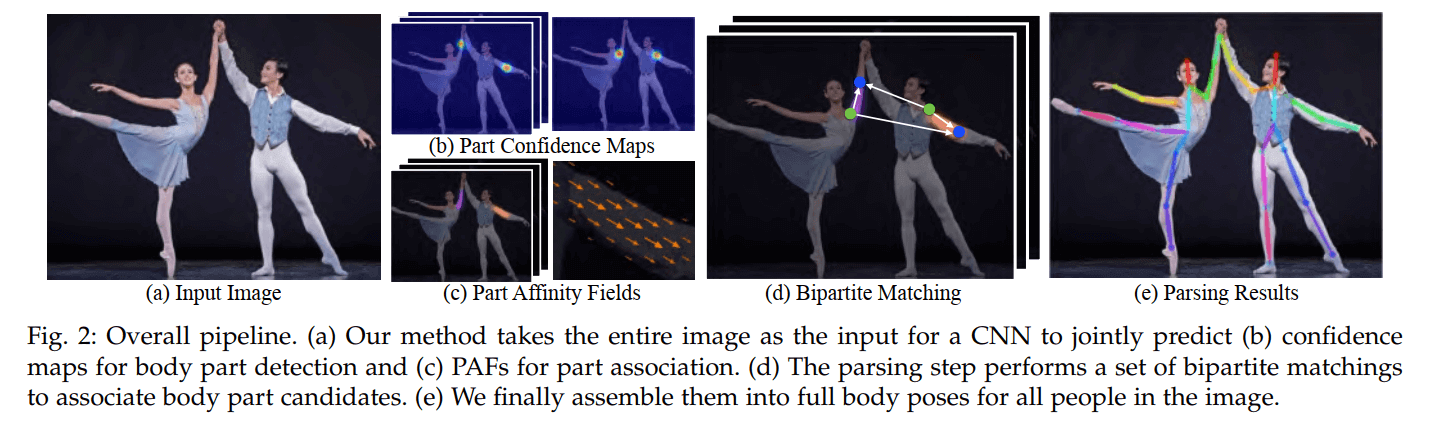
\includegraphics[scale=0.3]{chap3/c3_figs/pipeline.png}
\end{center}
\caption{Tổng thể kiến trúc}
\label{fig:pipelineS}
\end{figure}
\FloatBarrier

Hình 2 mình họa toàn bộ nội dung phương pháp. Hệ thống lấy đầu vào, một ảnh màu có kích thước wxh (hình 2a) và tạo ra ngõ ra, tọa độ của những keyponts cho mỗi cá nhân trong ảnh (hình 2e). Đầu tiên, một mạng CNN đồng thời dự đoán một loạt những confidence maps (cfm) S của những vị trí bộ phận cơ thể (hình 2b) và một loạt những miền vector 2D (vf) L của part affinities, cái mà mã hóa độ liên kết giữa các phần cơ thể (hình 2C). Tập hợp  có J cfm, một map cho mỗi bộ phận, trong đó . Tập hợp  có C vf, một cho mỗi chi, trong đó , mỗi vị trí ảnh trong Lc mã hóa một vector 2D (được show trong hình 1). Cuối cùng, cfm và affinity fields được phân tích bởi suy luận tham lam (hình 2d) để tạo ra các keypoints 2D cho tất cả người trong ảnh.

Phương pháp này đưa toàn bộ ảnh đầu vào qua một mạng CNN 2 nhánh để đồng thời dự đoán những confidence map cho sự detect phần cơ thể, thể hiện trong hình b, và part affinity fields cho sự liên kết các phần, thể hiện trong hình c. Bước phân tích thể hiện một loạt những liên kết giữa hai điểm (liên kết lưỡng cực) để liên kết những phần cơ thể (d). Cuối cùng, chúng tôi lắp ráp chúng lại với nhau tạo thành những tư thế cơ thể hoàn chỉnh cho tất cả những người trong ảnh (e).

\begin{itemize} % chấm đầu dòng
\item Đầu tiên, hình ảnh được truyền qua mạng cơ sở để trích xuất các bản đồ đặc trưng. Trong bài báo, tác giả sử dụng 10 lớp đầu tiên của mô hình VGG-19.
\end{itemize}


\begin{itemize} % chấm đầu dòng
\item Sau đó, các bản đồ tính năng được xử lý với nhiều giai đoạn CNN để tạo: một bộ Bản đồ tin cậy một phần và một bộ các trường có mối quan hệ một phần (PAF)
	\begin{itemize}
	\item \textbf{Confidence Maps} : một bộ bản đồ độ tin cậy 2D S cho các vị trí phần cơ thể. Mỗi vị trí chung có một bản đồ.
	\item \textbf{Part Affinity Fields} : một tập hợp các trường vectơ 2D L mã hóa mức độ liên kết giữa các phần.
	\end{itemize}
\end{itemize}


\begin{itemize} % chấm đầu dòng
\item Cuối cùng, \textbf{Confidence Maps} và \textbf{Part Affinity Fields} được xử lý bằng thuật toán tham lam để có được tư thế cho mỗi người trong ảnh.
\end{itemize}

\subsection{Các phần cụ thể}
%\renewcommand{\labelitemi}{$\square$}
%\renewcommand\labelitemii{$\nabla$}
%\renewcommand\labelitemiii{$\square$}
\begin{itemize}
  \item[$\square$] \textbf{Confidence Maps}
  Confidence Maps là một đại diện 2D cho niềm tin rằng một bộ phận cơ thể cụ thể có thể được đặt trong bất kỳ pixel nào. Với J là số lượng vị trí bộ phận cơ thể (khớp). Sau đó, \textbf{Confidence Maps} $S = (S_1, S_2, .., S_J)$ với $S_j \in R^{w \times h},j \in (1 \ldots J)$
  Tóm lại, mỗi bản đồ tương ứng với một khớp và có cùng kích thước với hình ảnh đầu vào .

  \item[$\square$] \textbf{Part Affinity Fields(PAF)}
  Trường quan hệ một phần \textbf{(PAF)} là một tập hợp các trường dòng mã hóa các mối quan hệ cặp đôi không cấu trúc giữa các bộ phận cơ thể.

Mỗi cặp bộ phận cơ thể có một \textbf{PAF} , tức là cổ, mũi, khuỷu tay, v.v.

Cho $C$ là số lượng các cặp phần trên cơ thể. Sau đó \textbf{PAFs} là các thiết lập \textbf{$L = (L_1, L_2, ..., L_c)$} với \textbf{$L_c \in R^{w \times h \times 2},c \in (1 \ldots C)$}

Nếu một pixel nằm trên một chi (phần cơ thể), giá trị trong $L_c$ tại pixel đó là một vectơ đơn vị 2D từ khớp bắt đầu đến khớp cuối.
\item[$\square$] \textbf{CNN nhiều giai đoạn}

\FloatBarrier
\begin{figure}[htp]
\begin{center}
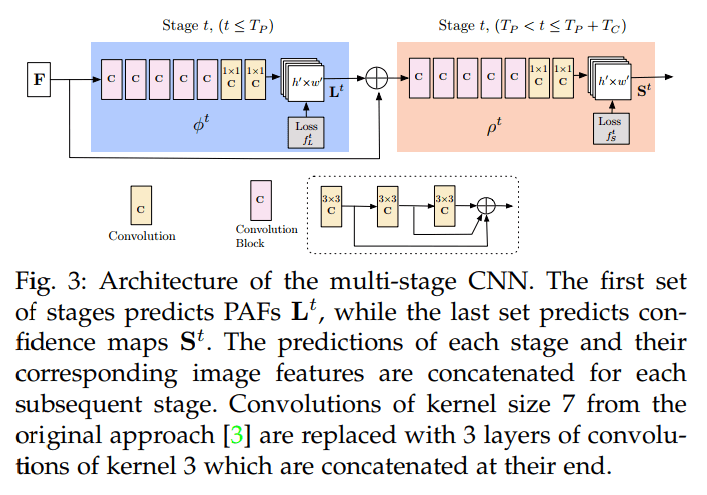
\includegraphics[scale=0.65]{chap3/c3_figs/CNN_m.png}
\end{center}
\caption{Kiến trúc của CNN nhiều giai đoạn từ phiên bản tạp chí của OpenPose}
\label{fig:pipelineS}
\end{figure}
\FloatBarrier

\textbf{CNN nhiều giai đoạn gồm các bước như sau:}
\begin{itemize}
\item Tính toán các \textbf{part affinity fields (PAFs)}, $ L^{1}$ từ feature maps của mạng cơ sở $F$. Cho $\phi^1$ là mạng CNN mạng CNN tại bước 1. 
$$L^1 = \phi^1(F) $$

\item Giai đoạn $t$ đến giai đoạn $T_P$: Tinh chỉnh dự đoán của \textbf{PAF} từ giai đoạn trước bằng cách sử dụng bản đồ tính năng $F$ và các \textbf{PAF} trước đó $(L^{t-1})$.Với $\phi^t$ là CNN ở giai đoạn t.
$$L^t = \phi^t(F, L^{t-1}), \forall 2 \leq t \leq T_P$$
\item Sau khi $T_P$ lặp đi lặp lại, quá trình được lặp lại việc phát hiện \textbf{confidence maps} , bắt đầu trong dự đoán PAF cập nhật mới nhất . $\rho^t$ là CNN ở giai đoạn $t$. Quá trình được lặp lại cho $T_C$.
$$S^{T_P} = \rho^t(F, L^{T_P}), \forall t = T_P$$
$$S^t = \rho^t(F, L^{T_P}, S^{t-1}), \forall T_P \leq t \leq T_P + T_C$$

\item Ma trận $S$ và $L$ cuối cùng là \textbf{Confidence Maps} và \textbf{part affinity fields (PAFs)} sẽ được xử lý thêm bằng thuật toán tham lam.

\end{itemize}
\end{itemize}
\textbf{Chú thích:}
CNN nhiều giai đoạn này là từ phiên bản tạp chí 2018. Trong phiên bản CVPR 2017 gốc, họ đã tinh chỉnh cả bản đồ độ tin cậy và các trường mối quan hệ một phần (PAF) ở mỗi giai đoạn. Do đó, họ đòi hỏi nhiều tính toán và thời gian hơn ở mỗi giai đoạn. Trong cách tiếp cận mới, tác giả nhận thấy rằng cách tiếp cận mới làm tăng cả tốc độ và độ chính xác tương ứng 200\% và 7\%.

\subsection{Phương pháp hồi quy}
\label{sss:MHD3_ly_thuyet_do_phuc_tap}

